\documentclass[12pt,a4paper,fleqn]{article}

%%%%%%%%%%%%%%%%%%%%%% LES PACKAGES
\input{packages_MP2I.tex}

%%%%%%%%%%%%%%%%%%%%%% MISE EN FORME
%%%%%%%%%%%%%%%%%%%%%%%%%%%%%%%%%%%%%%%%%%%%
% MISE EN FORME DU TITRE 
%%%%%%%%%%%%%%%%%%%%%%%%%%%%%%%%%%%%%%%%%%%%
\newcommand{\titreCopie}[2]{
\noindent
\textsc{Lettres Philosophie}
\hfill
#2
%\\%[0.4cm]
\begin{center}
\LARGE
\hrule
\vspace{.4cm}
#1 \\[0.4cm]
\hrule
\end{center}
\vspace*{0.4cm}
}

\newcommand{\titrecours}[1]{
\noindent
\begin{center}
\LARGE
\hrule
\vspace{.4cm}
#1 \\[0.4cm]
\hrule
\end{center}
\vspace*{0.4cm}
}

%%%%%%%%%%%%%%%%%%%%%%%%%%%%%%%%%%%%%%%%%%%%
% MISE EN FORME DES PIEDS DE PAGE
%%%%%%%%%%%%%%%%%%%%%%%%%%%%%%%%%%%%%%%%%%%%
\AtEndDocument{\label{lastpage}}
\lhead{}
\chead{}
\rhead{}
\lfoot{ 
Ryan Bouchou
}
\cfoot{}
\rfoot{\thepage/\pageref{lastpage}}
\renewcommand{\headrulewidth}{0pt}
\fancyhfoffset{0.7cm}



%%%%%%%%%%%%%%%%%%%%%%%%%%%%%%%%%%%%%%%%%%%%
% REMISE EN FORME DES SOUS-SOUS-SECTIONS  
%%%%%%%%%%%%%%%%%%%%%%%%%%%%%%%%%%%%%%%%%%%%

% section = exercices
%\renewcommand{\thesection}{\centering \arabic{section}}
% sous-section = question
%renewcommand{\thesubsection}{\arabic{subsection}}

\newcommand{\ssection}[1]{%
 
\begin{center}
    \hline
    
    \section*{\centering\normalfont\scshape #1}
    
    \hline
\end{center}
  }


\titleformat{\subsubsection}
   {\normalfont\fontsize{13pt}{13pt}\selectfont\bfseries}% apparence commune au titre et au numéro
   {\thesubsubsection}% apparence du numéro
   {1em}% espacement numéro/texte
   {}% apparence du titre

\titleformat{\subsubsubsection}
   {\normalfont\fontsize{11pt}{12pt}\selectfont\bfseries}% apparence commune au titre et au numéro
   {\thesubsubsubsection}% apparence du numéro
   {1em}% espacement numéro/texte
   {}% apparence du titre
%%%%%%%%%%%%%%%%%%%%%%%%%%%%%%%%%%%%%%%%%%%%
% MISE EN FORME DU CODE AVEC MINTED
%%%%%%%%%%%%%%%%%%%%%%%%%%%%%%%%%%%%%%%%%%%%

%pour le style des numéros de ligne minted
\renewcommand{\theFancyVerbLine}{\sffamily
\textcolor{expli}{\scriptsize
\oldstylenums{\arabic{FancyVerbLine}}}}

%pour éviter l'italique 
%car apparaissaient en italique à la fois les commentaires et les includes
\newtoggle{inminted}
\AtBeginEnvironment{minted}{\let\itshape\relax}

%paramètres pour le c
\setminted[c]{
	%--fond et cadre	
	bgcolor = black!3!white,
	frame = leftline,
	framesep = 6pt,
	rulecolor= expli,
	%--numéro de ligne
	linenos=true,
	numbersep=4pt,
	%stepnumber=2,
	xleftmargin=20pt,%pour que les chiffres débordent pas
	%--découpage des longues lignes
	breaklines=true,
	%--tabulations
	tabsize=2,
	}

%%
\setminted[csyntax]{
	%--fond et cadre	
	bgcolor = black!3!white,
	frame = leftline,
	framesep = 6pt,
	rulecolor= expli,
	%--numéro de ligne
	linenos=false,
	numbersep=4pt,
	%stepnumber=2,
	xleftmargin=20pt,%pour que les chiffres débordent pas
	%--découpage des longues lignes
	breaklines=true,
	%--tabulations
	tabsize=2,
	}

%paramètres pour le ocaml
\setminted[ocaml]{
	%--fond et cadre	
	%bgcolor = black!3!white,
	frame = leftline,
	framesep = 6pt,
	rulecolor= expli,
	%--numéro de ligne
	linenos=true,
	numbersep=4pt,
	%stepnumber=2,
	xleftmargin=20pt,%pour que les chiffres débordent pas
	%--découpage des longues lignes
	breaklines=true,
	%--tabulations
	tabsize=2,
	}

 %paramètres pour le ocaml
\setminted[bash]{
	%--fond et cadre	
	bgcolor = black!3!white,
	frame = leftline,
	framesep = 6pt,
	rulecolor= expli,
	%--numéro de ligne
	linenos=true,
	numbersep=4pt,
	%stepnumber=2,
	xleftmargin=20pt,%pour que les chiffres débordent pas
	%--découpage des longues lignes
	breaklines=true,
	%--tabulations
	tabsize=2,
	}








%%%%%%%%%%%%%%%%%%%%%%% LA PALETTE DE COULEURS
\input{palette_aef.tex}

%%%%%%%%%%%%%%%%%%%%%%% LES COMMANDES 
\input{commandes_MP2I.tex}

%%%%%%%%%%%%%%%%%%%%%%% LES "BOITES"
\newenvironment{p}{%
  \vspace*{0.5cm}
  \thmbox[S]{\textbf{Propriété}}%
  \hspace*{-1.5em}\slshape\ignorespaces%
  }
  {%
  \endthmbox\vspace*{1ex}%
  }
  
\newenvironment{df}[1]{%
  \vspace*{0.5cm}
  \thmbox[M]{\textbf{Définition:} #1}%
  \hspace*{-1.5em}\slshape\ignorespaces%
  }
  {%
  \endthmbox\vspace*{1ex}%
  }
  
\newenvironment{rp}[1]{%
  \vspace*{0.5cm}
  \thmbox[M]{\textbf{Rappel:} #1}%
  \hspace*{-1.5em}\slshape\ignorespaces%
  }
  {%
  \endthmbox\vspace*{1ex}%
  }

\newenvironment{pr}{%
  \vspace*{0.5cm}
  \thmbox[M]{\textbf{Proposition}}%
  \hspace*{-1.5em}\slshape\ignorespaces%
  }
  {%
  \endthmbox\vspace*{1ex}%
  }

  


\PassOptionsToPackage{svgnames}{xcolor}

\usepackage{tcolorbox}



\renewcommand*\contentsname{Sommaire}


\newcommand{\subsubsubsection}[1]{\paragraph{#1}\mbox{}\\}
\setcounter{secnumdepth}{4}
\setcounter{tocdepth}{4}


\usetikzlibrary{babel, backgrounds, calc, intersections, matrix, positioning}

\newlength{\myrulewidth}
\setlength{\myrulewidth}{0.4pt} % c'est la valeur par défaut de \pgflinewidth
\newlength{\myCellSize}
\setlength{\myCellSize}{0.7cm}

%%%%%%%%%%%%%%%%%%%%%%%
\newcounter{chapter}
\newcounter{thm}

\usepackage{mathtools, amssymb}
        \usepackage[thmmarks, amsmath]{ntheorem}
        %------------------------------------------------
        \theoremstyle{plain}
        \theoremheaderfont{\upshape\bfseries}
        \theorembodyfont{\itshape}
        \theoremseparator{\textbf{.\,---}}
        \newtheorem{theoreme}{Théorème}[chapter]
        \newtheorem{corollaire}[thm]{Corollaire}
        \newtheorem{lemme}[thm]{Lemme}
        %-----------------------------------------------
        \theoremheaderfont{\bfseries}
        \theorembodyfont{\mdseries\upshape}
        \theoremseparator{.}
        \theoremstyle{definition}
        \newtheorem{definition}{Définition}[chapter]
        \newtheorem{exemple}{Exemple}[chapter]
        \newtheorem{exo}{Exercice}[chapter]
        \newtheorem{propriete}{Propriété}[chapter]

        %------------------------------------------------
        \theoremstyle{nonumberplain}
        \theoremheaderfont{\mdseries\upshape}
        \theoremsymbol{$\mathrm{o}.\varepsilon.\delta.$}
        \theoremheaderfont{\scshape}
        \theoremseparator{\,:}
        \newtheorem{dem}{Démonstration}
    \setcounter{chapter}{1}
    \setcounter{thm}{1}

\usepackage{cleveref}
\crefformat{refth}{#2Théorème~#1#3}{}
\crefformat{refdef}{#2Définition~#1#3}{}
\crefformat{refrem}{#2Remarque~#1#3}{}
\crefformat{refdem}{#2Démonstration~#1#3}{}
\crefformat{refexo}{#2Exercice~#1#3}{}





%%%%%%%%%%%%%%%%%%%%%%%%%%%%%%%%%%%%%%%
\begin{document}
\pagestyle{fancy} %active les pieds de pages
\tcbset{colback=red!5!white,colframe=red!75!black,fonttitle=\bfseries}

%%%%%%%%%%%%%%%%%%%%%%%%%%%%%%%%%%%%%%%

\thispagestyle{empty}
\vspace*{0.7cm}
\begin{center}
    \begin{tikzpicture}
        \draw (0.2,-3) rectangle (15.9,-28 );
        \node[text width=6.2cm,font=\Huge] at (8,-10) {\centerline{\fontsize{32}{32}\selectfont ---  Cours d'Ocaml  ---}};
        \node[text width=6.2cm,font=\Huge] at (8,-12) {\centerline{\fontsize{18}{18}\selectfont \textit{RIPOPÉE INITIATIQUE}}};  
        \node[text width=6.2cm,font=\Huge] at (8,-23) {\centerline{\fontsize{18}{18}\selectfont RYAN BOUCHOU}};
    \end{tikzpicture}
\end{center}

%%%%%%%%%%%%%%%%%%%%%%%%%%%%%%%%%%%%%%%
\newpage
\tableofcontents
%%%%%%%%%%%%%%%%%%%%%%%%%%%%%%%%%%%%%%%%%%%%
\section{Les suites}
\subsection{Les suites arithmétiques}
\begin{definition}
    Soit $(u_n)_{n\in\mathbb{N}}$ une suite. On dit que $(u_n)$ est une \emph{suite arithmétique} si et seulement si $\exists r\in\mathbb{R} : \forall n\in\mathbb{N}, u_{n+1}-u_n=r$. Dans ce cas, on appelle $r$ la \emph{raison} de la suite.
\end{definition}
\begin{propriete}
    Soit $(u_n)_{n\in\mathbb{N}}$ une suite arithmétique de raison $r$. On a :
    $$\forall n\in\mathbb{N}, u_n=u_0+nr$$
\end{propriete}
\begin{propriete}
    Soit $(u_n)_{n\in\mathbb{N}}$ une suite arithmétique de raison $r$. On a :
    $$\forall n,p\in\mathbb{N} : p\leq n, u_n=u_p+(n-p)r$$
\end{propriete}
\subsubsection{Monotonie}
\begin{propriete}
    Soit $(u_n)_{n\in\mathbb{N}}$ une suite arithmétique de raison $r$ non nulle.
    $$\begin{cases}
        r>0 & (u_n) ~\text{est croissante}\\
        r<0 & (u_n) ~ \text{est décroissante}
    \end{cases}$$
\end{propriete}
\subsubsection{Somme de termes consécutifs}
La somme des $n$ termes consécutifs d'une suite arithmétique est donnée par la formule :
$$
S_n = \frac{n+1}{2} \cdot (a_0 + a_n)
$$

où $S_n$ est la somme des $n+1$ termes, $a_0$ est le premier terme, $a_n$ est le dernier terme et $n+1$ est le nombre de termes.

\subsection{Les suites géométrique}
\begin{definition}
    Soit $(u_n)_{n\in\mathbb{N}}$ une suite non nulle. On dit que $(u_n)$ est une \emph{suite géométrique} si et seulement si $\exists r\in\mathbb{R}^* : \forall n\in\mathbb{N}, \frac{u_{n+1}}{u_n}=q$. Dans ce cas, on appelle $q$ la \emph{raison} de la suite.
\end{definition}
\begin{propriete}
    Soit $(u_n)_{n\in\mathbb{N}}$ une suite géométrique de raison $q$. On a :
    $$\forall n\in\mathbb{N}, u_n=u_0*q^n$$
\end{propriete}
\begin{propriete}
    Soit $(u_n)_{n\in\mathbb{N}}$ une suite géométrique de raison $q$. On a :
    $$\forall n,p\in\mathbb{N} : p\leq n, u_n=u_p*q^{(n-p)}$$
\end{propriete}
\subsubsection{Monotonie}
\begin{propriete}
    Soit $(u_n)_{n\in\mathbb{N}}$ une suite géométrique de raison $q$ non nulle.\\
    Si $u_0$ est positif:
    $$\begin{cases}
        q>1 & (u_n) ~\text{est croissante}\\
        0<q<1 & (u_n) ~ \text{est décroissante}
    \end{cases}$$
    Si $u_0$ est négatif:
    $$\begin{cases}
        q>1 & (u_n) ~\text{est décroissante}\\
        0<q<1 & (u_n) ~ \text{est croissante}
    \end{cases}$$
\end{propriete}décroissante
\begin{propriete}
    Soit $(u_n)_{n\in\mathbb{N}}$ une suite géométrique de raison $q$ non nulle.\\
    $$\begin{cases}
        |q|>1 & (u_n) ~\text{est divergente}\\
        0<|q|<1 & (u_n) ~ \text{est convergente}\\
        q=1 & (u_n) ~\text{est constante}\\
        q=-1 & (u_n) ~\text{oscille entre}~u_0 ~\text{et}~ u_1
    \end{cases}$$
\end{propriete}
\subsubsection{Exemples graphiques}

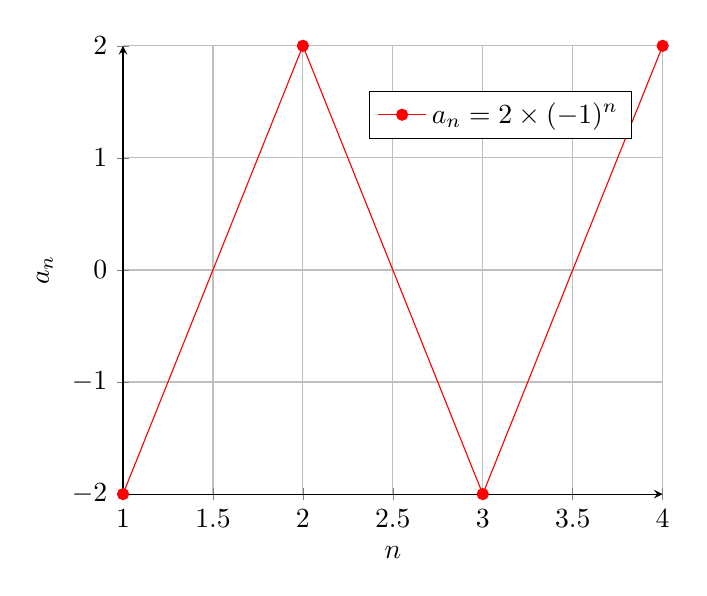
\begin{tikzpicture}
  \begin{axis}[
    xlabel={$n$},
    ylabel={$a_n$},
    axis lines=left,
    grid,
    mark=*,
    legend style={at={(0.7,0.9)},anchor=north}
  ]

  % Définition de la suite oscillante
  \def\a{2}
  \def\r{-1}
  
  % Calcul des premiers termes
  \pgfmathsetmacro{\aOne}{-\a}
  \pgfmathsetmacro{\aTwo}{\a}
  \pgfmathsetmacro{\aThree}{-\a}
  \pgfmathsetmacro{\aFour}{\a}

  % Tracé des points
  \addplot[red, mark=*] coordinates {(1, \aOne) (2, \aTwo) (3, \aThree) (4, \aFour)};
  \addlegendentry{$a_n = 2 \times (-1)^{n}$}

  \end{axis}
\end{tikzpicture}
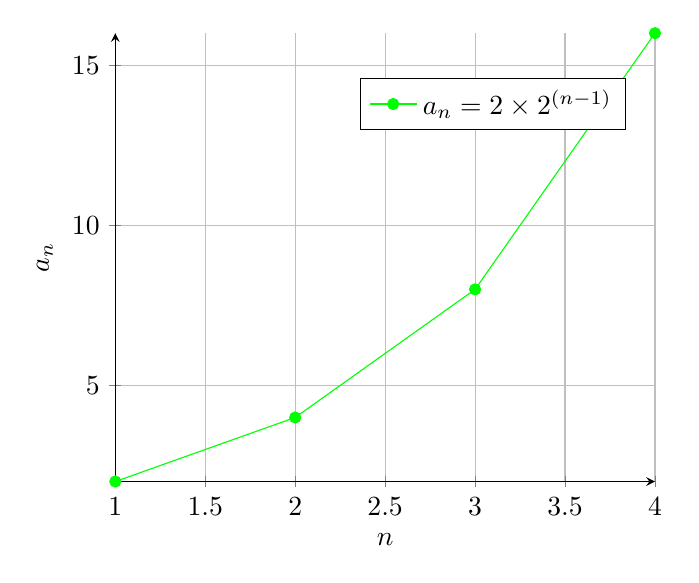
\begin{tikzpicture}
  \begin{axis}[
    xlabel={$n$},
    ylabel={$a_n$},
    axis lines=left,
    grid,
    mark=*,
    legend style={at={(0.7,0.9)},anchor=north}
  ]

  % Définition de la suite géométrique divergente
  \def\a{2}
  \def\r{2}
  
  % Calcul des premiers termes
  \pgfmathsetmacro{\aOne}{\a * \r^0}
  \pgfmathsetmacro{\aTwo}{\a * \r^1}
  \pgfmathsetmacro{\aThree}{\a * \r^2}
  \pgfmathsetmacro{\aFour}{\a * \r^3}

  % Tracé des points
  \addplot[green, mark=*] coordinates {(1, \aOne) (2, \aTwo) (3, \aThree) (4, \aFour)};
  \addlegendentry{$a_n = 2 \times 2^{(n-1)}$}

  \end{axis}
\end{tikzpicture}
\\[0.5cm]
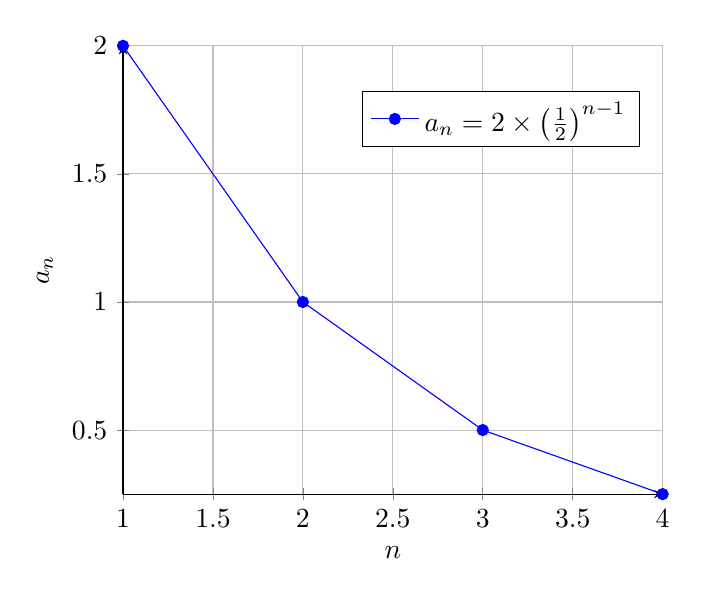
\begin{tikzpicture}
  \begin{axis}[
    xlabel={$n$},
    ylabel={$a_n$},
    axis lines=left,
    grid,
    mark=*,
    legend style={at={(0.7,0.9)},anchor=north}
  ]

  % Définition de la suite géométrique convergente
  \def\a{2}
  \def\r{0.5}
  
  % Calcul des premiers termes
  \pgfmathsetmacro{\aOne}{\a * \r^0}
  \pgfmathsetmacro{\aTwo}{\a * \r^1}
  \pgfmathsetmacro{\aThree}{\a * \r^2}
  \pgfmathsetmacro{\aFour}{\a * \r^3}

  % Tracé des points
  \addplot[blue, mark=*] coordinates {(1, \aOne) (2, \aTwo) (3, \aThree) (4, \aFour)};
  \addlegendentry{$a_n = 2 \times \left(\frac{1}{2}\right)^{n-1}$}

  \end{axis}
\end{tikzpicture}
\subsubsection{Somme de n termes consécutifs}
La somme de $n$ termes consécutifs d'une suite géométrique est donnée par la formule :
$$
\begin{cases}
    S_n = a_1 \cdot \frac{q^n - 1}{q - 1} & \text{si}~q\ne 1\\
    S_n =n\cdot a_1 & \text{sinon}
\end{cases}
$$
où\\
\begin{center}
    \begin{minipage}{0.4\textwidth}
    \begin{itemize}
    \item $S_n$ est la somme des $n$ termes consécutifs
    \item $a_1$ est le premier terme
    \end{itemize}
\end{minipage}
\begin{minipage}{0.4\textwidth}
    \begin{itemize}
    \item $r$ est la raison de la suite géométrique
    \item $n$ est le nombre de termes
    \end{itemize}
\end{minipage}
\end{center}
\newpage
\subsection{Récapitulatif sur les suites}
\begin{codeb}
    

\begin{enumerate}
    \item Une suite $\left(u_n\right)$ peut être définie de façon explicite : il existe alors une fonction $f$ définie sur $D_f$ telle que, pour tout entier $n \in D_f, u_n=f(n)$. Cela permet de:
    \begin{itemize}
        \flch modéliser une situation qui dépend de $n$;
        \flch calculer un terme quelconque de la suite en lien avec la situation.
    \end{itemize}
    \item Une suite $\left(u_n\right)$ à valeurs dans $\mathcal{D}_m$ peut être définie par récurrence : il existe alors une fonction $g$ définie sur $D_g$ telle que, pour tout $n \in \mathbb{N}, u_{n+1}=g\left(u_n\right)$. Cela permet de :
    \begin{itemize}
        \flch modéliser une situation dans laquelle un terme dépend du précédent.
    \end{itemize}
    \item $\left(u_n\right)$ est croissante à partir de $n=0$ lorsque, pour tout $n \in \mathbb{N}, u_{n+1} \geqslant u_n$ et $\left(u_n\right)$ est décroissante à partir de $n=0$ lorsque, pour tout $n \in \mathbb{N}, u_{n+1}\leq u_n$. Cela permet de:
    \begin{itemize}
        \flch trouver le sens de variation d'une suite;
        \flch résoudre des problèmes liés à des situations de variations.
    \end{itemize}
    \item Une suite est arithmétique lorsqu'il existe un réel $r$ tel que, pour tout $n \in \mathbb{N}, u_{n+1}=u_n+r$.
    
    Pour tous entiers naturels $n$ et $p, u_n=u_p+(n-p)\times r$ et, en particulier, $u_n=u_0+n r$.
    
    Une suite arithmétique de raison $r$ est croissante si $r>0$, décroissante si $r<0$ et constante si $r=0$.
    
    Pour tout entier naturel $n$ non nul, $1+2+\ldots+n=\frac{n(n+1)}{2}$. Cela permet :
    \begin{itemize}
        \flch étudier une situation de récurrence où un terme s'obtient à partir du précédent en ajoutant toujours le même nombre.
    \end{itemize}
\end{enumerate}
\end{codeb}



\section{Fondements}
Les mathématiques sont une discipline qui exige à la fois clarté, rigueur et originalité.
Ainsi, il convient de maîtriser un certain nombre de conventions afin de rendre son propos cohérent
et intelligible. Dans ce contexte, on se propose de présenter les notations usuelles nécessaires
à notre pratique des mathématiques.
\subsection{Les ensembles de nombres}
Les ensembles sont traités spécifiquement dans le chapitre \cref{ensembles}, pour autant, on procède
à un certain nombre de rappels ici.
\subsubsection{Ensembles usuels}
\begin{itemize}
    \item On appelle ensemble des \important{entiers naturels}, nôté $\mathbb{N}$, l'ensemble composé
    des nombres entiers positifs ou nuls.
    \item On appelle ensemble des \important{entiers relatifs}, nôté $\mathbb{Z}$, l'ensemble composé
    des entiers de signe quelconque. 
    \item On appelle ensemble des \important{rationnels}, nôté $\mathbb{Q}$, l'ensemble composé
    des nombres pouvant s'écrire sous la forme d'une fraction.
    \item On appelle ensemble des \important{décimaux}, nôté $\mathbb{D}$, l'ensemble composé
    des nombres à virgule.
    \item On appelle ensemble des \important{réels}, nôté $\mathbb{R}$, l'ensemble composé
    des nombres réels (\textit{i.e. quelconques})
    \item On appelle ensemble des \important{complexes}, nôté $\mathbb{C}$, l'ensemble composé
    des nombres complexes. (\textit{hors programme})
\end{itemize}
\begin{coder}
    De plus, on a l'inclusion suivante entre les ensembles précédemment cités:
$$\mathbb{N} \subset \mathbb{Z} \subset \mathbb{D} \subset \mathbb{Q} \subset \mathbb{R} \subset \mathbb{C}$$
\end{coder}
Par ailleurs, étant donné un ensemble $\mathbb{E}$ parmi les ensembles usuels, on introduit
les notations:
\begin{itemize}
    \item $\mathbb{E}^* = \mathbb{E}\setminus\{0\}$
    \item $\mathbb{E}^+$ l'ensemble des termes positifs ou nuls de $\mathbb{E}$.
    \item $\mathbb{E}^-$ l'ensemble des termes négatifs de $\mathbb{E}$.
\end{itemize}
Ce faisant, on a par exemple $\mathbb{R}^{*}_{+}$ l'ensemble des réels strictement positifs, $\mathbb{Z}^{*}$
l'ensemble des entiers relatifs privé de 0, et ainsi de suite. 
\subsubsection{Intervalles}
Considérons $a,b\in\mathbb{R}$ tels que $a \leq b$. Dès lors, on note:
\begin{itemize}
    \item $[a,b]$ l'ensemble des nombres réels compris entre $a$ et $b$ inclus. Autrement-dit
    l'ensemble des réels $x$ tels que $a \leq x \leq b$. 
    \item $]a,b]$ l'ensemble des nombres réels compris entre $a$ exclu et $b$ inclus. Autrement-dit
    l'ensemble des réels $x$ tels que $a < x \leq b$. De façon similaire, on définit $[a,b[ et ]a,b[$.
\end{itemize}
De plus, on définit les intervalles d'entiers. Considérons $a,b\in\mathbb{N}$ tels que $a \leq b$. 
Dès lors, on note:
\begin{itemize}
    \item $[\![a,b]\!]$ l'ensemble des nombres entiers compris entre $a$ et $b$ inclus. Autrement-dit
    l'ensemble des entiers $x$ tels que $a \leq x \leq b$. 
    \item $]\!]3;4]\!]$ l'ensemble des nombres entiers compris entre $a$ exclu et $b$ inclus. Autrement-dit
    l'ensemble des entiers $x$ tels que $a < x \leq b$. De façon similaire, on définit $[\![a,b[\![$ et $]\!]a,b[\![$.
\end{itemize}
On note $+\infty$ et $-\infty$ les infinis, $\infty$ par abus lorsque le signe est obvie, ainsi que
$\pm\infty$ lorsque l'on souhaite dénoter les deux cas. Par ailleurs, \important{lorsqu'un infinis constitue l'une des bornes
d'un intervalle, la borne qui lui est adjointe est nécessairement ouverte}. Par exemple, on note 
$[0,+\infty[=\mathbb{R}^+$.\\
\begin{codeb}
    \textbf{Remarque}
    \begin{itemize}
        \item Si $a,b\in\mathbb{R}$ et $a \leq b$ ; alors, $[b,a]=\emptyset$. Similairement pour les intervalles d'entiers.
        \item Si $a,b\in\mathbb{R}$ et $a = b$ ; alors, $[a,b]=\{a\}=\{b\}$. Similairement pour les intervalles d'entiers.
        \item Si $a,b\in\mathbb{N}$ et $a \leq b$ ; alors, $[\![a,b]\!]=\{a, a+1, \dots, b-1, b\}=\{x\in\mathbb{N} : a \leq x \leq b\}$.
    \end{itemize}
\end{codeb}
\subsection{Manipulation des symboles}
\textit{Pour la suite, on suppose fixé deux ensembles $I$ et $E$ tous deux non vides.}
\subsection{Famille}
Une famille est une fonction d'un ensemble $I$ dans un ensemble $E$ permettant
d'indexer les éléments de $E$ à partir de ceux de $I$. On la note $(x_i)_{i\in I}$,
ou $(x_i)$ lorsque l'indexation est obvie. De plus, $x_i$ est le $i^{eme}$ termes de la famille. 
\subsubsection{Sommation}
Lorsque l'on travaille sur des ensembles, nous pouvons être emmener à sommer leurs éléments. 
Si on considère une famille $(x_i)$ d'éléments de $E$, alors:
$$\sum_{i\in I}x_i \text{ est la somme des éléments } x_i, \text{ pour tout } i \text{ dans } I$$
\begin{codeb}
    \textbf{Remarque}\\
    \begin{itemize}
        \item Il est important de noter que le choix de i importe peu ; subséquemment, on a:
        $$\sum_{i\in I}x_i = \sum_{j\in I}x_j = \sum_{\beta \in I}x_{\beta}$$
        On dit que i est une \emph{variable muette}. En revanche, il est important de discerner
        ce qui est fixé et ce qui ne l'est pas. Conséquentiellement, $\sum_{i\in[1..i]}x_i$ n'a pas de sens.
        \item Lorsque $E$ est fini de cardinal $n$, on considère $I=\{1,\dots,n\}$. Dans le cas contraire, généralement $I=\mathbb{N}$. 
    \end{itemize}
    
\end{codeb}
\begin{exemple} Un somme usuelle pour illustrer le principe:
$$\sum_{k=1}^{n}k=1+2+\dots+n=\sum_{k\in[\![1,n]\!]}k=\frac{n(n+1)}{2}$$
\end{exemple}
\subsection{Logique}
La logique est une branche fondamentale des mathématiques qui sous-tend notre capacité à étayer nos raisonnements en formalisant la notion de démonstration. À ce titre, on dispose de plusieurs outils de rédaction afin de mettre en oeuvre nos démonstrations.
\begin{definition}
    On appelle \emph{proposition} un énoncé mathématique possédant une valeur de vérité, vrai ou faux.
\end{definition}
\begin{exemple}
    "\textit{Dans tout triangle rectangle, le carré de l’hypoténuse est égale à la somme
des carrés des deux autres côtés}" est une proposition vraie.
\end{exemple}
\begin{definition}
    On appelle \emph{axiome} une proposition admise comme vraie.
\end{definition}
\subsubsection{Opérateurs}
\subsubsubsection{Non, ou, et}
Les opérateurs logiques permettent de former des propositions par \emph{induction} en combinant d'autres propositions. Considérons deux propositions $P$ et $Q$.
\begin{itemize}
    \item \important{non $P$} : est la proposition constituée de la négation de $P$
    
    \begin{table}[h]
        \centering
        \begin{tabular}{@{ }c | c }
        P & $\lnot P$\\
        \hline 
        T & \textcolor{red}{F} \\
        F & \textcolor{red}{T} \\
        \end{tabular}
        \caption{Table de vérité de la négation}
        \label{tab:negation}
    \end{table}
    
    \item \important{$P$ ou $Q$} : est la proposition qui est vrai si au moins l'une de ses deux composantes l'est.
    
    \begin{table}[h]
        \centering
        \begin{tabular}{@{ }c@{ }@{ }c | c@{ }@{ }c@{ }@{ }c@{ }@{ }c@{ }@{ }c}
        P & Q &  & P & $\lor$ & Q & \\
        \hline 
        T & T &  &  & \textcolor{red}{T} &  & \\
        T & F &  &  & \textcolor{red}{T} &  & \\
        F & T &  &  & \textcolor{red}{T} &  & \\
        F & F &  &  & \textcolor{red}{F} &  & \\
        \end{tabular}
        \caption{Table de vérité de la disjonction}
        \label{tab:disjonction}
    \end{table}
    
    \item \important{$P$ et $Q$} : est la proposition qui est vrai si $P$ et $Q$ le sont toutes deux.
    \begin{table}[h]
        \centering
        \begin{tabular}{@{ }c@{ }@{ }c | c@{ }@{ }c@{ }@{ }c@{ }@{ }c@{ }@{ }c}
        P & Q &  & P & $\land$ & Q & \\
        \hline 
        T & T &  &  & \textcolor{red}{T} &  & \\
        T & F &  &  & \textcolor{red}{F} &  & \\
        F & T &  &  & \textcolor{red}{F} &  & \\
        F & F &  &  & \textcolor{red}{F} &  & \\
        \end{tabular}
        \caption{Table de vérité de la conjonction}
        \label{tab:conjontion}
    \end{table}
\end{itemize}
\newpage
\subsubsubsection{Implication et équivalence}
\begin{itemize}
    \item \important{$P\implies Q$} : est la proposition qui signifie que "si $P$ est vraie, alors $Q$ aussi" c'est à dire "P est fausse ou Q est vraie". On dit que \emph{$P$ implique $Q$}
    \begin{table}[h]
        \centering
        \begin{tabular}{@{ }c@{ }@{ }c | c@{ }@{ }c@{ }@{ }c@{ }@{ }c@{ }@{ }c}
        P & Q &  & P & $\rightarrow$ & Q & \\
        \hline 
        T & T &  &  & \textcolor{red}{T} &  & \\
        T & F &  &  & \textcolor{red}{F} &  & \\
        F & T &  &  & \textcolor{red}{T} &  & \\
        F & F &  &  & \textcolor{red}{T} &  & \\
        \end{tabular}
        \caption{Table de vérité de l'implication}
        \label{tab:implication}
    \end{table}
    \item \important{$P \Leftrightarrow Q$} : est la proposition qui signifie que $\big( $($P$ implique Q) et ($Q$ implique $P$)$\big)$. On dit que \emph{$P$ est équivalent $Q$}
    \begin{table}[h]
        \centering
        \begin{tabular}{@{ }c@{ }@{ }c | c@{ }@{ }c@{ }@{ }c@{ }@{ }c@{ }@{ }c}
        P & Q &  & P & $\Leftrightarrow$ & Q & \\
        \hline 
        T & T &  &  & \textcolor{red}{T} &  & \\
        T & F &  &  & \textcolor{red}{F} &  & \\
        F & T &  &  & \textcolor{red}{F} & T & \\
        F & F &  &  & \textcolor{red}{T} &  & \\
        \end{tabular}
        \caption{Table de vérité de l'équivalence}
        \label{tab:equiv}
    \end{table}
\end{itemize}
\begin{coder}
    L'implication et l'équivalence sont des \important{relations transitives}. Ainsi, si :
    \begin{itemize}
        \item ($P \implies Q$) et ($Q \implies R$) alors ($P \implies R$)
        \item  ($P \Leftrightarrow Q$) et ($Q \Leftrightarrow R$) alors ($P \Leftrightarrow R$)
    \end{itemize}
\end{coder}
\subsubsection{Réciproque et contraposée}
\begin{definition}
    La \emph{réciproque} de "$P$ implique $Q$" est "$Q$ implique $P$".
\end{definition}
\begin{definition}
    La \emph{contraposée} de "$P$ implique $Q$" est "non $Q$ implique non $P$".
\end{definition}
\begin{coder}
    \important{Une implication et sa contraposée sont équivalentes}. De fait, lorsque l'on souhaite montrer "$P$ implique $Q$", il peut être préférable de montrer "non $Q$ implique non $P$". On parle de \emph{raisonnement par contraposée}
\end{coder}
\subsubsection{Quantificateurs}
Lorsque l'on souhaite utiliser des variables dans nos raisonnements, il est nécessaire d'introduire celles-ci. Pour ce faire, on dispose de \emph{quantificateurs}. Considérons une propriété $P$ dépendant de $x\in \mathcal{D}$, notée $P(x)$.
\begin{itemize}
    \item Lorsque $P$ est vraie pour toute valeur de $x$, on note : $\forall x\in \mathcal{D}, P(x).$ Ici, la virgule succédant le quantificateur signifie "on a".
    \item Lorsque $P$ est vraie pour au moins une valeur de $x$, on note : $\exists \,x \in \mathcal{D}, P(x).$ Ici, la virgule succédant le quantificateur signifie "tel que".
\end{itemize}
%\section{Raisonnement par récurrence}
Le raisonnement par récurrence est une méthode de démonstration qui fait son apparition au $XVII^e$ siècle dans dans le \textit{Traité du triangle arithmétique} de Blaise Pascal. Le principe de récurrence repose sur le fondement inductif de $\mathbb{N}$ et s'énonce comme suit:
$$\biggl[\mathcal{P}(0)\wedge\Bigl(\forall n\in\mathbb{N},\bigl(\mathcal{P}(n)\Rightarrow\mathcal{P}(n+1)\bigr)\Bigr)\biggr]\Longrightarrow\bigl(\forall n\in\mathbb{N},\mathcal{P}(n)\bigr)$$
Autrement dit, \textbf{si} \important{$\boldsymbol{\mathcal{P}(0)}$ est vraie} \textit{(initialisation)} \important{et que} \important{$\boldsymbol{\forall n\in\mathbb{N}}$, si la propriété est vérifiée au rang n, elle l'est aussi au rang suivant} \textit{(hérédité)} ; \textbf{alors,} \important{la propriété est vrai pour tout entier}.
\subsection{Schéma de preuve}
On s'attachera à suivre le schéma de preuve suivant:
\begin{codeb}
    Démontrons par récurrence sur $n\in\NN$ la propriété $\mathcal{P}(n):" \text{\textit{propriété dépendant de n}} "$
    \begin{itemize}
        \item \textit{Initialisation:} Montrons $\mathcal{P}(0)$.
        \item \textit{Hérédité:} Soit $n\in\NN$, supposons $\mathcal{P}(n).$ Montrons $\mathcal{P}(n+1):" \text{\textit{pte au rang n+1}}"$.
        \item Ainsi, $\mathcal{P}(0)$ est vraie et pour tout $n\in\mathbb{N},\mathcal{P}(n)$ entraîne $\mathcal{P}(n+1)$. Donc, par principe de récurrence, $\mathcal{P}(n)$ est vraie pour tout $n\in\NN$.
    \end{itemize}
\end{codeb}
\begin{coder}
    \textbf{Remarques}
    \begin{itemize}
        \flch S'épargner une définition explicite de $\mathcal{P}$ peut parfois vous ralentir lors de l'hérédité plus qu'autre chose. D'ailleurs n ne doit pas être quantifié dans celle-ci. 
        \flch Ne pas oublier de fixer n dans un ensemble de définition convenable avant l'hérédité, en tenant compte du rang de l'initialisation.
        \flch Une fois rompu à l'exercice, nous serons tenté de rédiger plus brièvement; toutefois, la mention explicite du principe de récurrence et la conclusion de validité pour toute valeur de $\NN$ ne doivent pas être omises. Il ne faut donc pas s'arrêter après avoir montré $\mathcal{P}(n+1)$.
    \end{itemize}
\end{coder}
\begin{exemple}
Montrons par récurrence pour $n\geq1$, $\mathcal{P}(n): "\sum_{k=1}^{n} k = \frac{n(n+1)}{2}"$
\begin{itemize}
    \item \textit{Initialisation (\(n = 1\)):}
\[ 1 = \frac{1(1+1)}{2} ~~\text{, d'où} ~ \mathcal{P}(1).\] 
    \item \textit{Hérédité:} Supposons $\mathcal{P}$ pour un entier \(k\geq1\) fixé, i.e., $1 + 2 + 3 + \ldots + k = \frac{k(k+1)}{2}.$

Montrons la propriété au rang suivant:
\begin{align*}
1 + 2 + 3 + \ldots + k + (k+1) &= \frac{k(k+1)}{2} + (k+1) \\
&= \frac{k(k+1) + 2(k+1)}{2} \\
&= \frac{(k+1)(k+2)}{2} & \text{D'où} ~ \mathcal{P}(k+1).
\end{align*}
Ainsi, $\mathcal{P}(1)$ est vraie et pour tout $n\in\NNe,\mathcal{P}(n)$ entraîne $\mathcal{P}(n+1)$. Donc, par principe de récurrence, $\mathcal{P}(n)$ est vraie pour tout $n\in\NNe$.
\end{itemize}
\end{exemple}
\begin{exo}\label[refexo]{exo:0}
    Considérons $(u_n)_{n\in\NN}\in\NN^{\NN}$ telle que $\begin{cases}
        u_0=-267\\
        \forall n\geq0, u_{n+1}=u_n+61
    \end{cases}$\\[0.3cm]
    Montrer par récurrence sur $n\in\NN$ la propriété 
    $
    \mathcal{P}_n : "u_n=61n-267"
    $
\end{exo}
\begin{exo}\label[refexo]{exo:0bis}
    Considérons $(u_n)_{n\in\NNe}\in\NN^{\NNe}$ telle que $\begin{cases}
        u_1=1\\
        \forall n\geq1, u_{n+1}=\frac{n+1}{n}*u_n
    \end{cases}$\\[0.3cm]
    \begin{enumerate}
        \item Montrer par récurrence sur $n\in\NN$ la propriété 
    $
    \mathcal{P}_n : "u_n>0"
    $.
        \item De façon subsidiaire, en déduire que $(u_n)$ est décroissante.
    \end{enumerate}

\end{exo}
\begin{exo}\label[refexo]{exo:1}
    Montrer que $\sum_{k=1}^{n}k^2 = \frac{(k+1)(k+2)(2k+3)}{6}$
\end{exo}
\begin{exo}\label[refexo]{exo:2}
    Montrer que $(a + b)^n = \sum_{k=0}^{n} \binom{n}{k} a^{n-k} b^k$
\end{exo}
\subsection{D'autres types de récurrence}
\subsubsection{Récurrence d'ordre 2}
Lorsqu'on établit une propriété $\mathcal{P}(n)$ qui dépend de $\mathcal{P}(n-1)$ et $\mathcal{P}(n-2)$, alors il faut procéder comme suit:
\begin{codeb}
    Démontrons par récurrence sur $n\geq2$ la propriété $\mathcal{P}(n):" \text{\textit{propriété dépendant de n}} "$
    \begin{itemize}
        \item \textit{Initialisation:} Montrons $\mathcal{P}(0)$ et $\mathcal{P}(1)$.
        \item \textit{Hérédité:} Soit $n\in\NN$, supposons $\mathcal{P}(n)$ et $\mathcal{P}(n+1)$ Montrons $\mathcal{P}(n+2):" \text{\textit{pte au rang n+2}}"$.
        \item Ainsi, $\mathcal{P}(0)$ et $\mathcal{P}(1)$ sont vraies et pour tout $n\in\mathbb{N},\mathcal{P}(n)$ et $\mathcal{P}(n+1)$ entraînent $\mathcal{P}(n+2)$. Donc, par principe de récurrence, $\mathcal{P}(n)$ est vraie pour tout $n\in\NN$.
    \end{itemize}
\end{codeb}
\begin{exemple}
    Considérons la suite $(u_n)_{n\in\NN}\in\NN^{\NN}$ définie par $u_0=1, u_1=3$ et $\forall n\geq0, u_{n+2} = 4u_{n+1} - 3u_n$. On montre par récurrence d'ordre 2 sur $n\in\NN$ que $u_n = 3^n$.
\end{exemple}
\begin{coder}
    \textbf{Remarque}\\
    La preuve par récurrence se généralise à l'ordre $k\geq0$
\end{coder}
\subsubsection{Récurrence finie}
Cette récurrence s'établit sur un domaine de définition fini, par exemple $\intervalle{0}{K}$ où $K\in\NN$ est fixé.
\subsubsection{Récurrence forte}
On suppose la propriété vraie à tous les rangs précédents pour la montrer à un rang donné. Il suffit d’initialiser sur le premier terme.
\subsubsection{Récurrences multiples}
On opère simultanément des récurrences sur plusieurs variables. On imbrique en général les récurrences les unes dans les autres. Attention à bien énoncer les propriétés à démontrer pour chaque récurrence.
\subsection{Exercices}
\begin{exo}\label[refexo]{exo:5}
    Montrer que $\forall n\in \NNe,\sum_{k=0}^{n-1} 2k + 1  = n^2$
\end{exo}
\begin{exo}\label[refexo]{exo:6}
    Soit $a\in\mathbb{R}^+$. Montrer que pour $n\geq1$, 
    $$ (1 + a)^n \geq 1 + na $$
\end{exo}
\begin{exo}\label[refexo]{exo:7}
    Considérons la suite $(u_n)$ définie par $\begin{cases}u_0=1\\u_{n+1}=\sqrt{1+u_n} & \forall n\in \NN \end{cases}$
\end{exo}
\begin{exo}\label[refexo]{exo:8}
    Montrer pour $n\in\NNe$,
    $$S_n = \sum_{k=1}^{n} k^3 = 1^3+2^3+\ldots+n^3 = \dfrac{n^2(n+1)^2}{4}$$
\end{exo}
\begin{exo}\label[refexo]{exo:9}
    Considérons les propriétés:
    \begin{itemize}
        \item $\mathcal{P}_n :"4^n-1~\text{est divisible par 3}"$
        \item $\mathcal{Q}_n :"4^n+1~\text{est divisible par 3}"$
    \end{itemize}
    \begin{enumerate}
        \item Montrer que $\mathcal{P}_n$ est héréditaire.
        \item Montrer que $\mathcal{Q}_n$ est héréditaire.
        \item Montrer que $\mathcal{P}_n$ est vraie sur un domaine qu'on explicitera.
        \item Que dire de $\mathcal{Q}_n$?
    \end{enumerate}
\end{exo}
%\noindent\textbf{Correction \cref{exo:1}}
\begin{itemize}
    \item \textit{Initialisation (\(n = 1\)):}
\[1^2 = \frac{1(1+1)(2\cdot 1+1)}{6}\]
    \item \textit{Hérédité:} Supposons $\mathcal{P}_k$ pour un entier positif \(k\), i.e.,
\[1^2 + 2^2 + 3^2 + \ldots + k^2 = \frac{k(k+1)(2k+1)}{6}.\]

On veut montrer la propriété au rang \(k+1\):
\begin{align*}
1^2 + 2^2 + 3^2 + \ldots + k^2 + (k+1)^2 &= \frac{k(k+1)(2k+1)}{6} + (k+1)^2 \\
&= \frac{k(k+1)(2k+1) + 6(k+1)^2}{6} \\
&= \frac{(k+1)(k+2)(2k+3)}{6}.
\end{align*}
\end{itemize}




Donc, comme $\mathcal{P}_0$ est vraie et que pour tout entier positif \(n\), $\mathcal{P}_n$ entraine $\mathcal{P}_{n+1}$, on en déduit par récurrence que pour tout $n\in\NN$, $\mathcal{P}_n$ est vraie.\\[0.5cm]

\noindent\textbf{Correction \cref{exo:2}}\\
Montrons par récurrence sur $n\in\NN$ la formule du binome de Newton. Considérons deux réels \( a \) et \( b \),
$$
\mathcal{P}_n : "(a + b)^n = \sum_{k=0}^{n} \binom{n}{k} a^{n-k} b^k "
$$

\begin{itemize}
    \item \textit{Initialisation (\(n = 0\):)}
\[
(a + b)^0 = \binom{0}{0} a^0 b^0 = 1.
\]
    \item \textit{Hérédité:} Supposons $\mathcal{P}_k$ pour un entier positif \( k \), i.e.,
\[
(a + b)^k = \sum_{i=0}^{k} \binom{k}{i} a^{k-i} b^i.
\]

On veut montrer la propriété au rang \( k+1 \):
\begin{align*}
(a + b)^{k+1} &= (a + b)(a + b)^k \\
&= (a + b) \sum_{i=0}^{k} \binom{k}{i} a^{k-i} b^i \\
&= \sum_{i=0}^{k} \binom{k}{i} a^{k+1-i} b^i + \sum_{i=0}^{k} \binom{k}{i} a^{k-i} b^{i+1} \\
&= \binom{k}{0} a^{k+1} b^0 + \sum_{i=1}^{k-1} \binom{k}{i} a^{k+1-i} b^i + \binom{k}{k} a^0 b^{k+1} \\
&= \binom{k+1}{0} a^{k+1} b^0 + \sum_{i=1}^{k-1} \binom{k+1}{i} a^{k+1-i} b^i + \binom{k+1}{k+1} a^0 b^{k+1}.
\end{align*}
\end{itemize}
Donc, comme $\mathcal{P}_0$ est vraie et que pour tout entier positif \(n\), $\mathcal{P}_n$ entraine $\mathcal{P}_{n+1}$, on en déduit par récurrence que pour tout $n\in\NN$, $\mathcal{P}_n$ est vraie.\\[0.5cm]
\noindent\textbf{Correction \cref{exo:5}}\\
On utilise l'identité remarquable $(1+n)^2=1+2n+n^2$\\[0.5cm]
\noindent\textbf{Correction \cref{exo:6}}\\
On part de $\mathcal{P}_n$, on multiplie par $(1+a)$ et on utilise le fait que $a>0$.\\[0.5cm]
\noindent\textbf{Correction \cref{exo:7}}\\
Pour l'hérédité:
\begin{align*} 
u_n\leq u_{n+1} &\ssi u_n+1 \leq u_{n+1}+1 \\
&\ssi \sqrt{u_n+1} \leq \sqrt{u_{n+1}+1} &~croissance~de~x\mapsto\sqrt{x}\\
&\ssi u_{n+1} \leq u_{n+2}
\end{align*}

\noindent\textbf{Correction \cref{exo:8}}\\
Pour l'hérédité:\\
Soit un entier $n\geq1$. On suppose $\mathcal{P}_n$ vraie : $S_n = \displaystyle \sum_{k=1}^{n} k^3 = 1^3+2^3+\ldots+n^3 = \dfrac{n^2(n+1)^2}{4}$
\begin{align*}
S_{n+1}&=1^3+2^3+\ldots+n^3+(n+1)^3 \\
&=S_n+(n+1)^3 \\
&=\dfrac{n^2(n+1)^2}{4}+(n+1)^3\\
&=(n+1)^2 \times \left(\dfrac{n^2}{4}+n+1\right) \\
&=(n+1)^2\times \dfrac{n^2+4n+4}{4} \\
&=(n+1)^2\times \dfrac{(n+2)^2}{4}
\end{align*}

\noindent\textbf{Correction \cref{exo:9}}\\
Question 4: $4^n+1 \equiv 2~[3]$
%\section{Les ensembles}
\label{ensembles}
\subsection{Éléments généraux}
\begin{df}{Ensemble}
    Un ensemble est une collection d'objets appelés \textbf{éléments}, qui peuvent être en nombre fini ou non.
\end{df}
Un ensemble peut se définir de deux manières :
\begin{itemize}
    \item En donnant la liste explicite et exhaustive de ses éléments. (Raisonnablement dans le cas des ensembles finis)\\
    Exemple: $E=\{6,8,D,\%\}$
    \item Par compréhension : lorsque les éléments vérifient une propriété particulière.\\
    Exemple: $ E=\{x\in\mathbb{R} : x^{2}+x+1=0\} ~ i.e ~ Rac(X^{2}+X+1)$
\end{itemize}
\noindent
On note $\emptyset$ l'ensemble vide, ne contenant donc aucun élément. Par ailleurs, un certain nombre d'ensembles de références sont nécessaires ; à savoir: $(\mathbb{N},\mathbb{Z},\mathbb{Q},\mathbb{R},\mathbb{C})$
\noindent
On définit pour la suite E et F des ensembles quelconques, ainsi que $n\in\mathbb{N}^{*}$
\subsection{Opérations ensemblistes}
\begin{itemize}
    \item Appartenance: $x\in E$ si x appartient à E
    \item Inclusion: $E\subset F$ si E est inclus dans F ; i.e, E est un sous-ensemble de F
    \item Réunion: $E\cup F$ est l'ensemble des éléments appartenant à E ou F
    \item Intersection: $E\cap F$ est l'ensemble des éléments appartenant à E et à F
    \item Exclusion: $E\backslash F$ est l'ensemble des éléments de E qui n'appartiennent pas à F
    \item Différence symétrique: $E\triangle F$ est l'ensemble des éléments qui sont uniquement dans E et uniquement dans F. Autrement dit, $E\triangle F=(E\cup F)\backslash (E\cap F)$
\end{itemize}
Par ailleurs, on note P(E) \textbf{les parties de E}, l'ensemble des sous-ensembles de E.\\[0.3cm]
\warning ~ Si $B=\{1,7,8\}$ Attention à la différence entre $\{1\}\subset B ~et~ \{1\}\in P(B)$
\subsection{Cardinalité}
\begin{df}{Cardinal}
    On note Card(E), |E| ou encore \#E, le nombre d'éléments de E. On l'appelle \textbf{cardinal} de E.
\end{df}
\begin{df}{Ensembles deux à deux disjoints}
    Si $E_1,...,E_n$ sont deux à deux disjoints, alors $\forall i,j\in[1..n] ~ et ~i\neq j, Card((E_i\cap E_j))=0$
\end{df}
\begin{p}
    Si $E_1,...,E_n$ sont deux à deux disjoints et finis, alors $Card(E_1\cup ... \cup E_n)=\sum_{i=1}^{n}Card(E_i)$
\end{p}
\newpage
\subsection{Produit cartésien}
On appelle produit cartésien de n ensemble 
 $E_1,...,E_n$, l'ensemble \begin{center}
     $E_1\times...\times E_n=\{(x_1,...,x_n) ~|~ x_1\in E_1,...,x_n\in E_n\}$
 \end{center}
 dont les éléments sont des n\_uplets. On parle alors de couple, triplet, quadruplets etc...\\
 Si l'un des $E_i$ est vide alors, le produit cartésien l'est aussi. Enfin, si $E_1=...=E_n=E$ alors on note leur produit cartésien $E^{n}$

\begin{p}
    Soient $E_1,...,E_n$ des ensembles finis.\\
    $Card(E_1\times...\times E_n)=\prod\limits_{i=1}^n Card(E_{i})$
\end{p}
\subsection*{Exercices}
\subsubsection*{Exercices 1}
On considère le diagramme de Venn suivant, avec A,B,C trois parties d'un ensemble E;~et a,b,c,d,e,f,g,h des éléments de E.\\[.5cm]
\begin{minipage}{0.5\textwidth}
    \includegraphics[scale=2]{venn.png}
\end{minipage}
\begin{minipage}{0.5\textwidth}
    Dire si les affirmations suivantes sont vraies ou fausses:
    \begin{itemize}
        \item $g\in A\cap \bar B$
        \item $g\in\bar A\cap \bar B$
        \item $g\in\bar A\cup\bar B$
        \item $f\in C\backslash A$
        \item $e\in \bar A\cap\bar B\cap \bar C$
        \item $\{h,b\}\subset \bar A\cap\bar B$
    \end{itemize}
\end{minipage}
\subsubsection*{Exercice 2}
Soient 
A
,
B
,
C
 trois ensembles tels que 
A
$\cup$
B
=
B
$\cap$
C
. Montrer que 
A
$\subset$
B
$\subset$
C
.


\subsubsection*{Exercice 3}
Soient 
A
, 
B
 et 
C
 trois parties d'un ensemble 
E
. Pour 
X
$\subset$
E
, on note 
$X^c$
 le complémentaire de 
X
 dans 
E
. Démontrer les lois de Morgan suivantes :\\
\begin{center}
    \begin{array}{lll}
\mathbf{1.}\ (A\cap B)\cup C=(A\cup C)\cap (B\cup C)&&\mathbf{2.}\ (A^c)^c=A\\
\mathbf{3.}\ (A\cap B)^c=A^c\cup B^c&&\mathbf{4.}\ (A\cup B)^c=A^c\cap B^c.\\
\end{array}
\end{center}

\subsubsection*{Exercice 4}
Écrire l'ensemble des parties de E={a,b,c,d}.
\subsubsection*{Exercice 5}
On considère l'ensemble $D=\{(x,y)\in\mathbb R^2;\ x^2+y^2\leq 1\}$. Montrer qu'il ne peut pas s'écrire comme un produit cartésien de deux parties de $\mathbb{R}$. 
\subsubsection*{Exercice 6}
On considère $\sum_1 =\{0,1\}$ et  $\sum_2 =\{a,b,c,d,e\}$. On souhaite composer des mots de passes composé d'un chiffre et de 8 lettres. Quel est le nombre de mdp possibles ?\\ Quel est le nombres de mots de passes si on s'autorise à avoir un ou deux chiffres ?
\section{Dénombrement}
On considère dans cette partie un ensemble E de cardinal fini n et $0\leq k\leq n$:
\subsection{k\_Arrangements}

\begin{df}{Arrangement}
    On appelle k\_liste ou k\_Arrangements un k\_ uplet d'éléments de E tous différents. 
\end{df}
On assimile un k\_Arrangement au nombre d'issues lors d'un tirage sans remise de k éléments dans un ensemble à n éléments.
\begin{p}
    Le nombre de k\_Arrangements vaut $n(n-1)\dots (n-k+1)=\frac{n!}{(n-k)!}$
\end{p}
\begin{p}
    Le nombre de permutations de E vaut $n!$
\end{p}

\subsection{Combinaisons}
\begin{df}{k\_Combinaison}
    Partie de E à k éléments. 
\end{df}
On assimile le nombre de k-combinaison au nombre d'issues d'un tirage avec remise de k éléments dans un ensemble de cardinal n.
\begin{p}
    Le nombre de k-combinaisons de E est $\binom nk=\frac{n!}{k!(n-k)!}$\\
    Symétrie des coefficients binomiaux: $\binom nk=\binom n{n-k}$
\end{p}
\subsubsection*{Exercice 7}
On considère une course de karting comprenant n pilotes. Déterminer le nombre de podium possibles (on classera les 3 premiers).
\subsubsection*{Exercice 8}
On considère une course de karting comprenant n pilotes. Malheureusement, tous ne peuvent pas s'élancer sur la grille de départ en même temps. Déterminer le nombre de possibilités de sélectionner les k premiers qui partiront en premiers.  
\subsection{Triangle de Pascal}


\begin{center}
    
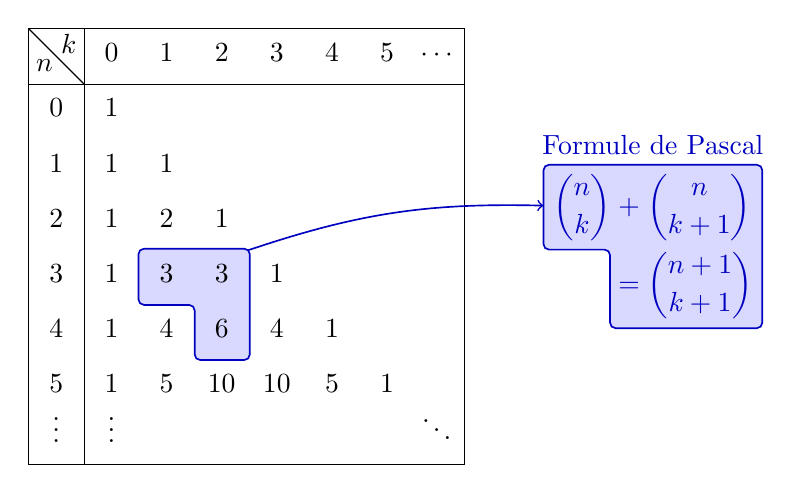
\begin{tikzpicture}[my rule/.style={line width=\myrulewidth},
                    my outline color/.initial=blue!75!black,
                    my text/.style={
                      color/.expanded={\pgfkeysvalueof{/tikz/my outline color}}},
                    my arrow/.style={
                      ->, line width=0.6pt,
                      draw/.expanded={\pgfkeysvalueof{/tikz/my outline color}}},
                    my highlight/.style={
                      draw/.expanded={\pgfkeysvalueof{/tikz/my outline color}},
                      fill=blue!15, line width=0.6pt, rounded corners=2pt}]

\matrix (mat) [
  my rule, draw, inner sep=0, matrix of math nodes,
  nodes={minimum width=\myCellSize,
         text height=0.6\myCellSize, text depth=0.4\myCellSize}]
  {
    \raisebox{-0.8ex}{$n$}\kern 0.3em\raisebox{0.7ex}{$k$}
           & 0      & 1 & 2 & 3 & 4 & 5   &[-2pt] \cdots \\
    0      & 1                                           \\
    1      & 1      & 1                                  \\
    2      & 1      & 2 & 1                              \\
    3      & 1      & 3 & 3  & 1                         \\
    4      & 1      & 4 & 6  & 4  & 1                    \\
    5      & 1      & 5 & 10 & 10 & 5 & 1                \\[-2pt]
    \vdots & \vdots &   &    &    &   &   &       \ddots \\
  };

\begin{scope}[my rule]
\draw (mat-1-1.north east) -- (mat-8-1.south east);
\draw (mat-1-1.south west) -- (mat-1-8.south east);
\draw ([shift={(0.5\myrulewidth, -0.5\myrulewidth)}]mat-1-1.north west) --
      (mat-1-1.south east);
\end{scope}

\path[my text] node [right=1cm of mat, label=above:{Formule de Pascal}]
  (formula)
  {%
    $\begin{aligned}
      \binom{n}{k} &\mathrel{+} \binom{n}{k+1} \\
                   &=           \binom{n+1}{k+1}
    \end{aligned}$%
  };

\begin{scope}[on background layer]
  \path[name path=p, my highlight]
    (mat-5-3.north west) -| coordinate (A)
    (mat-6-4.south east) -|
    (mat-5-3.south east) --
    (mat-5-3.south west)
    -- cycle;

  \pgfmathsetlengthmacro{\myWidth}{width("$\displaystyle \binom{n}{k}$")}
  \pgfmathsetlengthmacro{\myTotalHeight}{
    height("$\displaystyle \binom{n}{k}$") +
    depth("$\displaystyle \binom{n}{k}$")}
  \pgfmathsetlengthmacro{\myXshift}{\pgfkeysvalueof{/pgf/inner xsep} + \myWidth}
  \pgfmathsetlengthmacro{\myYshift}{\myTotalHeight +
                                    2*\pgfkeysvalueof{/pgf/inner ysep}}

  \path[my highlight]
    (formula.north west) -|
    (formula.south east) -|
    ([shift={(\myXshift,-\myYshift)}]formula.north west) coordinate (B) --
    (formula.north west |- B) --
    cycle;
  % Pour que la flèche parte vraiment de la bordure arrondie de p, il faut
  % ruser un peu. D'abord, il nous faut le point de départ :
  \path[name path=s] ([shift={(-10pt,-10pt)}]A) -- (A);
  \path[name intersections={of=p and s}];
\end{scope}

% Ensuite, on peut tracer la flèche.
\path[my arrow] (intersection-1) to[bend left=10]
                ($(formula.north west)!0.5!(formula.west)$);
\end{tikzpicture}
\end{center}
\subsubsection*{Démonstrations}
\begin{itemize}
    \flch\textbf{Méthode combinatoire}\\[5cm]
    \flch\textbf{Méthode algébrique}\\[5cm]
\end{itemize}




\newpage 
\begin{p}
    Pour n un entier natural, on a :$\sum_{k=0}^n=\binom{n}{k}=2^n$
\end{p}
\subsubsection*{Démonstrations}
\begin{itemize}
    \flch\textbf{Méthode combinatoire}\\[5cm]
    \flch\textbf{Méthode algébrique}\\[5cm]
\end{itemize}
\begin{p}
    Le nombre de parties d'en ensemble à n éléments vaut $2^n$
\end{p}
\subsubsection*{Exercice - Spécialité NSI}
\textit{On pourra aborder ici quelques notions sur les Langages}\\[0.3cm]
On considère $\sum_1 =\{0,1\}$ et  $\sum_2 =\{a,b,c,d,e\}$. On souhaite composer des mots de passes à partir du langage engendré par $L=\sum_{1}^{+} .\sum_{2}^{+}$ ; dont on restreindra leur taille à un entier n>1. On notera L' le langage subséquent. 
\begin{itemize}
    \item \textbf{Cas où n=2}\\
     Préciser la partie de L, notée L', qui nous intéresse ici à l'aide d'une description ensembliste par compréhension.\\
     Même question avec un produit cartésien. Donner alors le cardinal de cet ensemble. 
     \item \textbf{Cas où n>1}\\
     On considère u un mot de L'. Préciser sa décomposition et les caractéristiques de celles-ci.\\
     Donner le cardinal de L' en fonction de n, et des autres données de l'exercice. 
\end{itemize}




%%%%%%%%%%%%%%%%%%%%%%%%%%%%%%%%%%%%%%%%%%%%

\section{TD}
\begin{enumerate}
    \item Limite et continuité\hfill\pageref{tdlim}
    \item Ensemble et dénombrement\hfill\pageref{tdEns}
\end{enumerate}
\ssection{Limites et continuité}
\label{tdlim}
\noindent
On considère dans tout ce qui suit une fonction $f$ de $I\subset\mathbb{R}\rightarrow\mathbb{R}$ et $a\in \Bar{I}$\\
\subsection{Rappels de cours}
\subsubsection{Voisinage}
Analogie avec les suites et la condition "à partir d'un certain rang".
\begin{df}{Voisinage de a $\in\mathbb{R}$}
    On dit que $f$ vérifie une propriété $\mathcal{P}$ au voisinage de a ssi $\exists ~ \varepsilon >0 : f$ vérifie $\mathcal{P}$ sur $I\cap [a-\varepsilon,a+\varepsilon]$
\end{df}
\begin{df}{Voisinage de a $=\infty$}
    On dit que $f$ vérifie une propriété $\mathcal{P}$ au voisinage de +$\infty$ ssi $\exists ~ M\in\mathbb{R}: f$ vérifie $\mathcal{P}$ sur $I\cap [M,+\infty[$
\end{df}
\noindent
On notera $\mathcal{V}(a)$ l'ensemble des voisinages de a. Dans $\mathbb{R}, \{[a-\eta,a+\eta], \eta\in\mathbb{R}\}$ forme une base de $\mathcal{V}(a)$. Ce faisant, tout voisinage de a peut s'écrire sous cette forme. 

\subsection{Limites}

\subsubsection{Question de cours}
On considère un réel $l$. Traduisez les assertions suivantes:\\[0.5cm]
\begin{minipage}{0.5\textwidth}
    \begin{itemize}
        \item $f$ tend vers $l$ en a.
        \item $f$ tend vers $l$ en $+\infty$.
\end{itemize}
\end{minipage}
\begin{minipage}{0.5\textwidth}
    \begin{itemize}
        \item $f$ tend vers $+\infty$ en a.
        \item $f$ tend vers $+\infty$ en $+\infty$.
\end{itemize}
\end{minipage}


\subsubsection{Démonstrations}
\vspace*{-0.5cm}
\begin{pr}
    Si $f$ admet une limite finie en a, alors $f$ est bornée au voisinage de a.
\end{pr}
\begin{enumerate}
    \item Démontrer la propriété précédente.
    \item Démontrer le théorème d'unicité de la limite.
\end{enumerate}
    \subsubsection{Exercices}
\begin{enumerate}
    \item Démontrer que la fonction sinus n'admet pas de limite en l'infini
    \item Montrer que $\sqrt{x^{2}+1}-x \underset{x\to +\infty}{\longrightarrow} 0$
    \item La fonction $f= \left\{
    \begin{array}{ll}
        e^{\frac{-1}{x}} & \mbox{si } x>0 \\
        0 & \mbox{sinon.}
    \end{array}$ est-elle continue sur $\mathbb{R}$?
    \item Soit $f:\mathbb R\to\mathbb R$. On suppose que $f$ admet une limite $\ell$ en $+\infty$, avec $\ell>0$. Démontrer qu'il existe un réel $A>0$ tel que, pour tout $x\geq A$, $f(x)>0$.
    \item Soit $f:\mathbb R\to\mathbb R$ périodique et admettant une limite finie $l$ en $+\infty$. Montrer que $f$ est constante.
\end{enumerate}

\begin{df}{Sinus et cosinus hyperbolique}
    On définit sur $\mathbb{R}$ les fonctions sh : $x\rightarrow \frac{e^{x}-e^{-x}}{2}$ et ch : $x\rightarrow \frac{e^{x}+e^{-x}}{2}$
\end{df}
\subsubsection{Autour de $e^x$}
\begin{enumerate}
    \item Résoudre les systèmes d'équations suivantes : 
$$\begin{array}{lll}
\mathbf{1.}\ \left\{
\begin{array}{rcl}
e^xe^y&=&10\\
e^{x-y}&=&\frac 25
\end{array}
\right.&\quad\quad&\mathbf{2.}\ 
\left\{
\begin{array}{rcl}
e^x-2e^y&=&-5\\
3e^x+e^y&=&13
\end{array}\right.\\
\mathbf{3.}\ \left\{
\begin{array}{rcl}
5e^x-e^y&=&19\\
e^{x+y}&=&30
\end{array}
\right.
\end{array}$$
\item Démontrer que, pour tout $n\geq 2$, on a 
$$\left(1+\frac 1n\right)^n \leq e\leq \left(1-\frac 1n\right)^{-n}.$$

\item Démontrer que, pour tous $x,y\in\mathbb{R}$, $$sh(x+y)=sh(x)ch(y)+ch(x)sh(y)$$

\item Montrer que, pour tout $x\neq 0$,
$$\sum_{k=0}^n ch(kx)=\frac{ch(nx/2)sh\big((n+1)x/2\big)}{sh(x/2)}.$$
\end{enumerate}
\subsubsection{Retour sur les limites..}
\begin{enumerate}
    \item Montrer que: $\lim\limits_{x\rightarrow l}f(x)=+\infty \Longleftrightarrow \forall (x_n)\in I^{\mathbb{N}} ~ |~ x_n \underset{n\to +\infty}{\longrightarrow} l, ~ f(x_n)\underset{n\to +\infty}{\longrightarrow} +\infty$
    \item \textit{Variante} - Soit $f:\mathbb R \rightarrow \mathbb R$ périodique. Montrer qu'elle ne peut pas avoir de limite infinie en $+\infty$
    \item Déterminer les limites des fractions rationnelles suivantes:
\end{enumerate}
$$\begin{array}{lll}
\mathbf{1.} ~ \frac{X^2-X+1}{7X^3}~en~+\infty
&\quad\quad&\mathbf{2.}\ 
\frac{X^2+4e^X}{e^X}~en~+\infty\\[0.5cm]
\mathbf{3.} ~ x^{\frac{1}{1-x}} ~ en~1
&\quad\quad&\mathbf{4.}\ \lim\limits_{x \rightarrow 0^+} \left(\left(1+\dfrac{1}{\sqrt{x}}\right) (x-3)\right)

\end{array}
$$
%--------------------------------------------
% REMISE EN FORME DES SOUS-SOUS-SECTIONS  
%--------------------------------------------

% section = exercices
\renewcommand{\thesection}{Exercice~\arabic{section}}
% sous-section = question
\renewcommand{\thesubsection}{Question~\arabic{subsection}}
%--------------------------------------------

\ssection{Ensemble et dénombrement}
\label{tdEns}
\tocless\section{Formalisme des ensembles}
\tocless\subsection{Cours} 
\begin{minipage}{0.5\textwidth}
    \begin{itemize}
        \item $\pi\ldots\mathbb{Q}$
        \item $8.5\ldots\mathbb{R}$
        \item $\{6\}\ldots\mathbb{Z}$
        \item $(7,-9,5.8)\ldots~\ldots\ldots\ldots$
    \end{itemize}
\end{minipage}
\begin{minipage}{0.5\textwidth}
    \begin{itemize}
        \item $\mathbb{Q}\ldots\mathbb{R}$
        \item $\mathbb{N}\ldots\mathbb{Z}$
        \item $\mathbb{R}\ldots\mathbb{Z}$
        \item $\mathbb{R}^*\ldots\mathbb{R}$
    \end{itemize}
\end{minipage}
\tocless\subsection{Cours}Rappeler la définition d'un ensemble formulé par compréhension
\tocless\subsection{}
\begin{itemize}
    \item Donner l'ensemble des entiers naturels pairs
    \item Donner l'ensemble des entiers relatifs impairs
    \item Donner l'ensemble des entiers relatifs dont le reste de leur division par 3 vaut 2
    \item Soit $(n,S)\in\mathbb{N}^2$. Donner l'ensemble des n\_uplets dont la somme de leurs éléments vaut S.
\end{itemize}
\tocless\subsection{}
Soient $A=\{1,2,3\}$ et $B=\{0,1,2,4\}$. Donner les ensembles $A\cap B, A\cup B$ et $A\times B$
\tocless\subsection{}
Déterminer deux 3\_uplets de {0,1}. Combien en existe-t-il au total?
\tocless\subsection{}
Soient $A=[0,2]$ et $B=]1.5,3]$. Donner les ensembles $A\cap B, A\cup B$
\tocless\subsection{}
Soient A, B et C trois parties d'un ensemble E. Pour X$\subset$E, on note $X^c$ le complémentaire de X dans E. Démontrer les lois de Morgan suivantes :\\
\begin{center}
    \begin{math}
    \begin{array}{lll}
        \mathbf{1.}\ (A\cap B)\cup C=(A\cup C)\cap (B\cup C)&&\mathbf{2.}\ (A^c)^c=A\\
        \mathbf{3.}\ (A\cap B)^c=A^c\cup B^c&&\mathbf{4.}\ (A\cup B)^c=A^c\cap B^c.\\
    \end{array}
    \end{math}
\end{center}

\newpage
\tocless\section{Propriétés sur les ensembles}
\tocless\subsection{}
Soient $A=\{1,2,3\}$ et $B=\{0,1,2,4\}$. Donner $\#A, \#B, \#A\cup B$
\tocless\subsection{}
On réalise un sondage sur un ensemble d'individus afin de connaître les langages qu'ils maîtrisent. On reporte les résultats sur le diagramme de Venn suivant:\\[0.5cm]
\begin{minipage}{0.5\textwidth}
    \includegraphics[]{Imgs/images.jpg}
\end{minipage}
\begin{minipage}{0.5\textwidth}
Pour chacune des questions, on donnera une notation ensembliste afin de traduire l'énoncer. 
    \begin{itemize}
        \item Donner le nombre total de personnes interrogées.
        \item Donner le nombre d'individus qui parlent Anglais, Espagnol et Italien.
        \item Donner le nombre d'individus qui parlent Espagnol et Italien seulement.
        \item Donner le nombre d'individus qui parlent (Anglais et Italien) ou (Anglais et Espagnol)
    \end{itemize}
\end{minipage}
\tocless\subsection{}
Soient A et B deux ensembles finis et disjoints. On sait que Card(A$\cup$B)=23 et Card(A×B)=132. Déterminer Card(A) et Card(B) sachant que Card(A)<Card(B).
\tocless\section{Dénombrement}
\tocless\subsection{}
\begin{itemize}
    \item Combien y-a-t-il de podiums possibles?
    \item Combien y-a-t-il de podiums possibles où Émile est premier?
    \item Combien y-a-t-il de podiums possibles dont Émile fait partie?
    \item On souhaite récompenser les 3 premiers en leur offrant un prix identique à chacun. Combien y-a-t-il de distributions de récompenses possibles?
\end{itemize}
\tocless\subsection{}
Un cadenas possède un code à 3chiffres, chacun des chiffres pouvant être un chiffre de 1 à 9.
\begin{itemize}
    \item Combien y-a-t-il de codes possibles?
 \item Combien y-a-t-il de codes se terminant par un chiffre pair?
 \item Combien y-a-t-il de codes contenant au moins un chiffre 4?
 \item Combien y-a-t-il de codes contenant exactement un chiffre 4?
\end{itemize}
Dans cette question on souhaite que le code comporte obligatoirement trois chiffres distincts.
\begin{itemize}
     \item Combien y-a-t-il de codes possibles?
\item Combien y-a-t-il de codes se terminant par un chiffre impair?
 \item Combien y-a-t-il de codes comprenant le chiffre 
6
?
\end{itemize}


\newpage
%--------------------------------------------
% REMISE EN FORME DES SOUS-SOUS-SECTIONS  
%--------------------------------------------

% section = exercices
\renewcommand{\thesection}{\arabic{section}}
% sous-section = question
\renewcommand{\thesubsection}{\arabic{subsection}}
%--------------------------------------------
\section{Bibliographie}
\href{https://www.annales2maths.com/ts_exercices_rec1/}{Récurrence}
\end{document}
